\chapter{Physical Unclonable Function: classification and characterisation}
\label{ch:1-puf}


In this section, we will discuss in more detail about the typical design of \acrshort{puf}, how they work, and how we can evaluate their performance.

\begin{figure}[H]
    \centering
    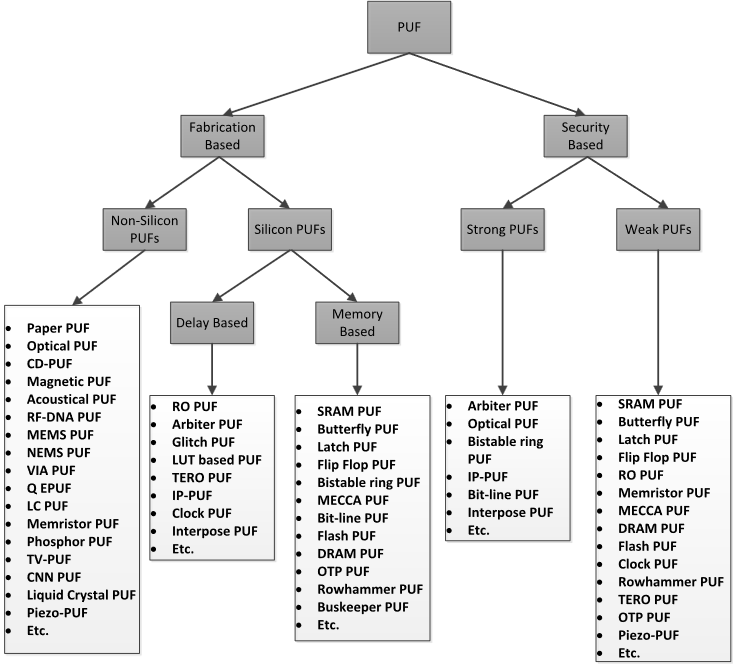
\includegraphics[width=0.84\linewidth]{images/full_puf_overview.png}
    \caption{\acrshort{puf} classification (from~\cite{anandakumar_fpga-based_2021})}
    \label{fig:PUF_ALL}
\end{figure}

The \acrshort{puf} concept was introduced in 2001 by \cite{pappu_physical_2001, pappu_physical_2002}, first addressed as \acrfull{powf}, as a comparison to the one-way functions based on number theory used in cryptography. The aim is to exploit randomness in the physical properties of a system to generate a binary sequence. As a first proof of concept, they used a transparent epoxy containing bubbles as the physical medium, which was 'read' by a laser at a specific angle to generate a pattern from the interference between the beam and the epoxy/bubble.\\

This has led to a variety of different designs which can be classified in two ways, as shown in figure~\ref{fig:PUF_ALL}: how they work physically (manufacturing based) and how they should be used (safety based).

\section{Fabrication based classification}

%FPAG-based \acrshort{puf} -> Also good for security

The non-silicon \acrshort{puf}s are \acrshort{puf}s implemented on systems such as optical, mechanical or magnetic systems. These will not be covered in this study and we will concentrate only on \acrfull{spuf}. The first introduction of \acrshort{spuf} was made by \cite{gassend_silicon_2002} in 2002, originally called \acrfull{sprf}. The advantage of such \acrshort{puf}s is the ease with which they can be integrated into other electronic circuits.\\

In general, electronic circuit models are expected to have some small number of defects in the silicon due to the limited precision of the manufacturing process. The defects are required to have a negligible effect on the device's operation, and this is a constraint that designers consider while designing such circuits. However, these effects can still be exhibited using appropriately designed circuits. These defects cannot be replicated with a similar precision manufacturing process and are often considered to be unknowable (in the sense that to be able to observe them directly one would generally need to destroy the \acrfull{ic}) and appear to be random. This means that they are properties that can be used to implement a \acrshort{puf} on an electronic circuit.\\

A wide range of methods can be utilised to expose these tiny manufacturing errors and to turn them into usable responses, i.e. binary values. There are two classes of methods based on how they exploit randomness: delay-based \acrshort{puf} and memory-based \acrshort{puf}. Designs using more than one \acrshort{puf} technique are called hybrid \acrshort{puf}.\\

Delay-based \acrshort{puf}s exploit small variation in the delay of electronic signals between two similar paths. In an ideal scenario, the two paths should produce identical delays, but in reality, there will always be slight differences in delay. These differences are typically small, and their influence on a typical electronic circuit is minimal. Delay-based \acrshort{puf} are electronic circuits designed to amplify these differences to the point where they dominate and determine the output response, ideally without any other external factor influencing the result.\\

Memory-based \acrshort{puf}s exploit transient state of memory elements during power-up and then observe which stable states they eventually transition to, resulting in the generation of the response.\\


\section{Security based classification}

A second way of classifying \acrshort{puf} is to separate them on the basis of the size of their \acrfull{crp} space. Some \acrshort{puf}s provide only one possible response. In this case, it can be considered that there is no input since the challenge corresponding to the only response is intrinsic to the \acrshort{puf} itself. Whereas, other \acrshort{puf}s have a large set of \acrfull{crp} spaces. This classification is helpful in determining how a \acrshort{puf} can be utilized for security applications.\\

Weak \acrshort{puf} are the \acrshort{puf}s with a small \acrshort{crp} space, with the extreme case being a \acrshort{puf} with only one response (the challenge is therefore not required as an input, as it is implicit in the \acrshort{puf} itself). These \acrshort{puf}s must be used in a secure environment and the \acrshort{crp} should not be revealed; otherwise, an attacker could record the entire CRP, compromising the security of the system. Thefore, these \acrshort{puf}s can only be used for applications such as key extraction, truly random number generation, or identification.\\

Strong \acrshort{puf} refers to \acrshort{puf}s with a large \acrshort{crp} space. In this case, revealing a few \acrshort{crp} does not compromise the \acrshort{puf} because there are still many of them that are unknown (in the ideal case where \acrshort{crp}s are not correlated in any way so that the remaining \acrshort{crp} cannot be predicted). Strong PUFs are ideal for use in authentication processes.


\section{Example of FPGA-based PUFs}


\subsection{Arbiter PUF}

\acrfull{apuf} are the most common and most studied of the \acrshort{puf}s.\\
The concept was introduced in 2002 \cite{gassend_silicon_2002} and many different versions have been created since then. It consists of two paths that travel through successive stages, where the 2 paths have 2 possible configurations depending on the input. The output is generated based on which path is globally the fastest due to the imperfections in the IC. This can be achieved by using successive stages of \acrfull{mux} that select which path the signal will take, as shown in figure~\ref{fig:APUF}.\\
Thus, this is a delay-based \acrshort{puf}, and since the number of \acrshort{crp} doubles for each additional stage, it is a strong \acrshort{puf}.

\begin{figure}[H]
    \centering
    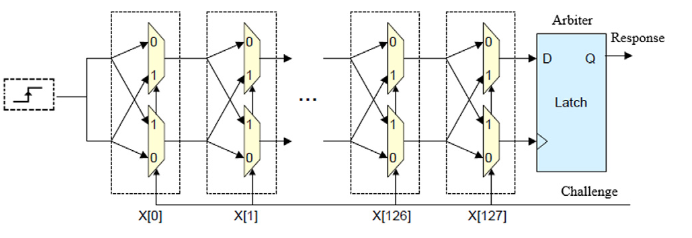
\includegraphics[width=0.75\linewidth]{images/APUF_diagram.png}
    \caption{Arbiter \acrshort{puf} diagram \cite{anandakumar_fpga-based_2021}}
    \label{fig:APUF}
\end{figure}

One concern with this design is the possibility to model the internal delay of each stage configuration to be able to predict the entire \acrshort{crp} space. A proposed countermeasure for this issue was presented in 2004 \cite{lee_technique_2004}, where feed-forward signals from the intermediate stage are used as input for some of the following stages. This approach is commonly known as a \acrfull{ffapuf}.\\

\begin{figure}[H]
   \begin{minipage}[b]{0.6\linewidth} 
        \centering
        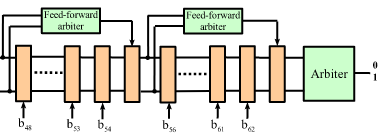
\includegraphics[width=\linewidth]{images/FF-APUF_Lee and al 2004.png}
        \caption{\acrshort{ffapuf} \cite{lee_technique_2004}}
        \label{FFAPUF}
   \end{minipage}\hfill
   \begin{minipage}[b]{0.35\linewidth}   
        \centering
        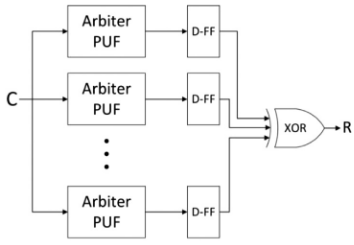
\includegraphics[width=\linewidth]{images/XOR-APUF Al-Hajj and al. 2021.png}
        \caption{\acrshort{xorapuf} \cite{el-hajj_taxonomy_2021}}
         \label{XORAPUF}
   \end{minipage}
\end{figure}

An alternative approach is to introduce an XOR layer at the output to enhance the confidentiality of the internal properties. This was studied by \cite{suh_physical_2007} in 2007, called a \acrfull{xorapuf}.\\

Since then, several other features have been developed and tested. To enhance the reliability, \cite{he_highly_2020} has proposed a \acrfull{bstapuf}. A more recent example is the work of \cite{anandakumar_implementation_2022} in 2022, which obfuscates the challenges and adds a majority voting system before the XOR. A comprehensive compilation of Arbiter \acrshort{apuf} was done by \cite{el-hajj_taxonomy_2021} in 2021.



\subsection{Ring oscillator PUF}

The design proposed by \cite{gassend_silicon_2002} does not directly evaluate the delay difference between two configurable paths. Rather, the signals were looping back into the same configurable path, thus forming an oscillating circuit. The frequency difference served as the measured parameter for determining the output. This was done in order to reduce the influence of the process variation on the output parameter.\\

\begin{figure}[H]
    \centering
    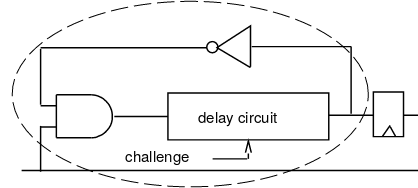
\includegraphics[width=0.6\linewidth]{images/RO_origine_Gassend_al_2002.png}
    \caption{Oscillating circuit using APUF for delay \cite{gassend_silicon_2002}}
    \label{fig:RO_ORIGINAL}
\end{figure}

This concept led to the development of another \acrshort{puf} design: the \acrfull{ropuf}. An oscillating circuit is designed using a basic delay element and replicated to form a collection of oscillators. All oscillators are compared to each other, and a '0' or a '1' is generated based on the oscillator with the fastest frequency.

\begin{figure}[H]
    \centering
    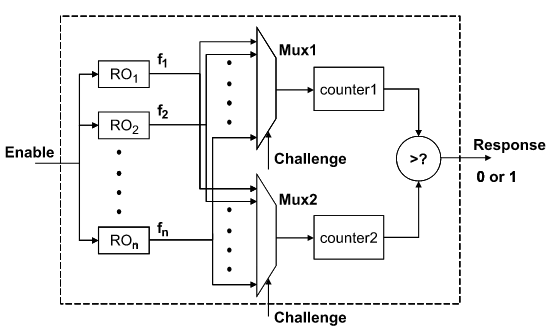
\includegraphics[width=0.7\linewidth]{images/RO_GENE_ORIGI_maiti_2009.png}
    \caption{\acrshort{ropuf} diagram \cite{maiti_improved_2009}}
    \label{fig:ROPUF}
\end{figure}

This concept was first studied in 2009 by \cite{maiti_improved_2009} using a \acrshort{sram} based \acrshort{fpga} (Spartan 3), then in 2017 by \cite{mureddu_efficient_2017} with a flash based \acrshort{fpga} (Microsemi SmartFusion2). In both cases, the oscillator circuit is made up of an AND gate (for control) and an odd number of NOT gates (for delay).\\

In 2022, \cite{yao_m-ro_2022} demonstrated the possibility of replacing the inverter-based oscillator with a \acrshort{mux}-based one, resulting in the creation of the \acrfull{mropuf}.

\begin{figure}[H]
    \centering
    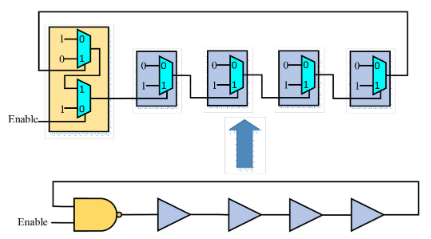
\includegraphics[width=0.7\linewidth]{images/MUX_ROPUF_YAO.png}
    \caption{\acrshort{mropuf} \cite{yao_m-ro_2022}}
    \label{fig:MUXROPUF}
\end{figure}

Similarly to the \acrshort{apuf}, \acrshort{ropuf} are delay-based \acrshort{puf}s. They can be considered weak or strong \acrshort{puf} depending on the oscillator circuit designs as well as the structure used to generate the output from the collection of oscillators.


%ResumeHere

\subsection{Transient effect ring oscillator PUF}
\label{subsubsec:intr_tero_puf}

The \acrshort{ropuf} concept has been proven to be often very vulnerable to physical attack and frequency analysis by \cite{clavier_frequency_2009} in 2009, \cite{bochard_true-randomness_2010} in 2010, \cite{hutchison_contactless_2012} in 2012 and \cite{bossuet_ultra-lightweight_2015} in 2015. Moreover, \cite{bochard_true-randomness_2010} also proved that the different oscillator cells of \acrshort{ropuf} are sensitive to locking phenomena (cells are not independent).\\

To avoid the locking phenomena and make the frequencies less accessible, a new design using transient effect has been proposed by \cite{bossuet_puf_2014} in 2014.\\
In \acrfull{teropuf}, the cells oscillation occurs in an unstable state and both the stabilisation time and the final number of oscillations are unpredictable. This can be achieved with the circuit represented in figure~\ref{fig:TEROPUF}, which is an \acrfull{sr-latch} with the set and reset signal combined. This design is also sometimes called \acrfull{ocpuf}

\begin{figure}[H]
    \centering
    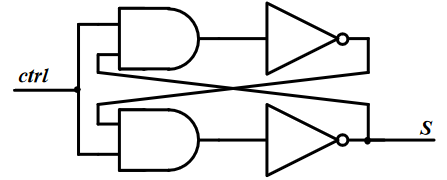
\includegraphics[width=0.5\linewidth]{images/TEROPUF.png}
    \caption{\acrshort{teropuf} diagram \cite{bossuet_puf_2014}}
    \label{fig:TEROPUF}
\end{figure}

The first design by \cite{bossuet_puf_2014} was tested on an Altera Cyclone II then by \cite{marchand_design_2016} on Altera Cyclone V and Xilinx Spartan 6 FPGAs.\\

The oscillator circuit has also been build using \acrshort{sr-latch} in \cite{habib_implementation_2017} and D-Latches in \cite{della_sala_novel_2021}, called \acrfull{ddpuf}.\\

\begin{figure}[H]
    \centering
    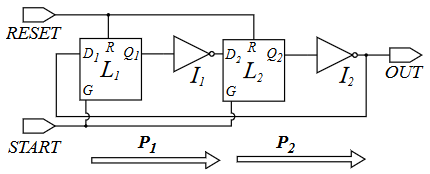
\includegraphics[width=0.5\linewidth]{images/DDPUF.png}
    \caption{\acrshort{ddpuf} diagram \cite{della_sala_novel_2021}}
    \label{fig:DDPUF}
\end{figure}

The idea of a programmable delay line using LUT input-output latency was re-introduced in 2018 by \cite{ardakani_improving_2018} on Spartan 3E and a high \acrshort{crp}s implementation ($2^{3N}$) has been proposed by \cite{zhang_highly_2020} in 2020 on an Altera DE2-115.\\

In 2019, \cite{tebelmann_side-channel_2019} studied the robustness of \acrshort{teropuf} design against side channels analysis. While it shows that \acrshort{teropuf} can still be vulnerable to some extent, it has also proposed a few countermeasures to minimise it. \acrshort{teropuf} still appear as one of the most promising delay based \acrshort{puf}.



\subsection{SRAM PUF}

In parallel to the evolution of delay based \acrshort{spuf}, the memory based \acrshort{spuf} development started with the \acrfull{srampuf} from \cite{paillier_fpga_2007} in 2007.\\
When an \acrshort{sram} element is powered up, its initial state is not one of the two stable ones ('1' and '0') but an unstable equilibrium in between. If none of the two stable states is forced, the state in which it will end up is unpredictable and is a function of the exact properties of the silicon.

\begin{figure}[H]
    \centering
    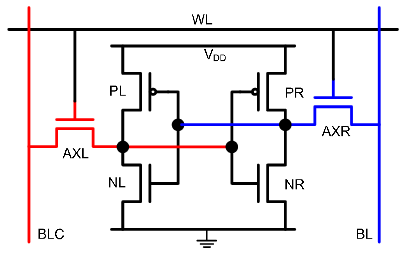
\includegraphics[width=0.45\linewidth]{images/SRAM.png}
    \caption{SRAM cell \cite{paillier_fpga_2007}}
    \label{fig:SRAM}
\end{figure}

This design has to advantage of using standard \acrshort{sram} chips, which are typically available in most of electronic board.\\
There have been multiple implementations since then, such as \cite{chen_fpga_2018} in 2008, who built a \acrfull{prng} from it, or \cite{usmani_applications_2018} in 2008 that used the variation of the \acrshort{puf} due to the temperature to create a temperature sensor with secured data values.\\


To eliminate the requirement of power up the \acrshort{sram} each time the \acrshort{puf} needs to be evaluated, \cite{cicek_new_2022} proposed in 2022 to introduce a \acrfull{rwcsrampuf}, violating in purpose the recommended operation of the \acrshort{sram}.


\subsection{Butterfly PUF}

For \acrshort{srampuf}, the \acrshort{fpga} needs to support uninitialised \acrshort{sram} memory, which is not always the case. To remove this requirement, \cite{kumar_extended_2008} introduced their \acrfull{bpuf} in 2008. The concept is the same that the \acrshort{srampuf} but the memory structure used is a cross-coupled latch that can be forced to an unstable state. 


\begin{figure}[H]
    \centering
    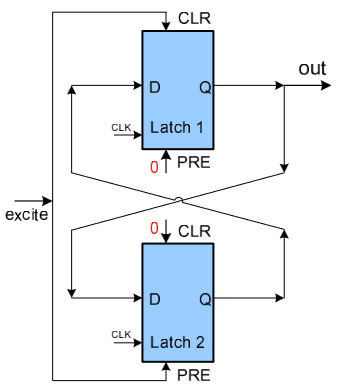
\includegraphics[width=0.45\linewidth]{images/BPUF.png}
    \caption{BPUF \cite{kumar_extended_2008}}
    \label{fig:BPUF}
\end{figure}


\subsection{Flip-Flop PUF}

Similarly to the \acrshort{bpuf}, the \acrfull{ffpuf} aims at removing the requirement on specific hardware from the \acrshort{srampuf}. Introduced in 2008 by \cite{maes_intrinsic_2008}, this \acrshort{puf} read the power-up value from D Flip-Flop.

\newpage
\subsection{Hybrid PUF}

It is also possible to combine two or more \acrshort{puf} techniques to have a more complex system that exploits the random defects in multiple ways. This can be useful to obtain a \acrshort{puf} that is more difficult to predict using \acrfull{ml} techniques. For example, \cite{devika_fpga_2022} has proposed in 2022 an implementation using both \acrshort{apuf} and \acrshort{bpuf} together.

\begin{figure}[H]
    \centering
    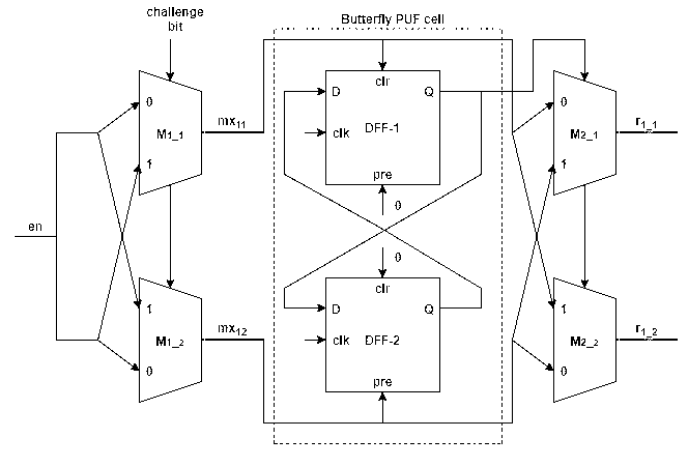
\includegraphics[width=\linewidth]{images/hybrid.png}
    \caption{Hybrid \acrshort{puf} diagram \cite{devika_fpga_2022}}
    \label{fig:HYBRID}
\end{figure}

\newpage
\section{Metrics}

To characterise and compare the performance of a \acrshort{puf}, multiple metrics have been used. In this section, we will see the main metrics used to evaluate the performance of \acrshort{puf} for security applications. The metrics that are computed on the set of responses of a single device are called intra-device metrics, and those that characterise the difference between the responses of different devices are called inter-device metrics.

\subsection{Uniformity}

The \acrfull{unif} is a measure of distribution between "0" and "1" bits in the response of a given device (intra-device). Ideally equal to 50\% to maximise the entropy.

\begin{equation}
    UF = \frac{1}{n} \sum_{i=1}^{n} r_i \times 100\%
\end{equation}

Where $n$ is the size of the response and $r_i$ is the $i$th bit of it.

\subsection{Reliability}


The \acrfull{relia} is a measure of the stability of the response of a given device (intra-device). Ideally equal to 100\% meaning that the response's bits are always the same.

\begin{equation}
     RE = 100\% - \frac{1}{s} \sum_{i=1}^s \frac{\mathrm{HD}\left(X_{ref}, X_i\right)}{n} \times 100 \% \\
\end{equation}

Where $s$ is the number of responses generated, $HD(X_{ref}, X_i)$ is Hamming distance between the $i$th response generated and the reference response.\\

The \acrfull{ber} can be obtained using only the right term of the sum.\\

This can be further improved using \acrfull{ecc} or \acrshort{bst} as done in \cite{he_highly_2020, he_highly_2021}.

\subsection{Bit-Aliasing}

The \acrfull{bit-alia} is a measure of how likely a bit value is to be '1' over all the devices (inter-device). This can reveal a bias in the implementation i.e. the response's bits are influenced by the implementation itself. Ideally, the distribution of bit-aliasing over different devices should follow a normal distribution centred around 50\%.

\begin{equation}
    BA_j = \frac{1}{k} \sum_{j=1}^{k} r_{i,j} \times 100\%
\end{equation}

Where $n$ is the number of bits of the response, $k$ is the number of devices and $r_{i,j}$ is the $i$th bit of the $j$th device response.

\subsection{Uniqueness}

The \acrfull{uniq} is a measure of how different the responses of different devices are (inter-device). Ideally equal to 50\%.

\begin{equation}
    UQ =\frac{2}{k(k-1)} \sum_{i=1}^{k-1} \sum_{j=i+1}^k \frac{\mathrm{HD}\left(X_i, X_j\right)}{n} \times 100\%
\end{equation}

Where $k$ is the number of devices, $\mathrm{HD}\left(X_i, X_j\right)$ the Hamming distance between the response word of device $i$ and $j$.


\newpage
\section{State of the art}
\label{sec:SOACompa}

The metrics just described are useful to compare the performance of different implementations. The table~\ref{tab:soa_impl} reports the performance of some of the \acrshort{fpga} implementation describes up to now. Not all studies have used the 4 metrics described here, and the implementations are done using different \acrshort{fpga}. The goal of this table is not to have a complete collection of \acrshort{puf}s implementation, only to have an overview of the typical performance that can be reached currently.\\

\begin{table}[H]
    \centering
    \begin{tabular}{|c|c|c|c|c|c|c|c|}
         \hline
         \textbf{method} & \textbf{\acrshort{relia}} & \textbf{\acrshort{unif}} & \textbf{\acrshort{uniq}} & \textbf{\acrshort{bit-alia}} & \textbf{device} & \textbf{Ref}\\
         \hline\hline
         \acrshort{apuf} & 99.55\% & 51.84\% & 46.21\% & -  & Artix-7 & \cite{anandakumar_implementation_2022}\\
         \hline
         \acrshort{ffapuf}& 90.2\% & - & 38\% & - & ASIC & \cite{lee_technique_2004}\\
         \hline
         \acrshort{xorapuf} & 99.41\% & 50.73\% & 48.69\% &  - & Artix-7 & \cite{anandakumar_implementation_2022}\\
         \hline
         \acrshort{bstapuf} & 99.99\% & - & 49.1\% & 50.3\% &  Artix-7 & \cite{he_highly_2020}\\
         \hline
         \acrshort{ropuf} & 100\% & - & 45.9\% & - &  Spartan-3 & \cite{maiti_improved_2009}\\
         \hline
         \acrshort{ropuf} & 99.19\% & 51.01 & 47.86\% & 51.01\% & Artix-7 & \cite{de_weerdt_implementation_2021}\\
         \hline
         BST-\acrshort{ropuf} & 99.99\% & 46.78\% & 48.64\% & - & Artix-7 & \cite{he_highly_2021}\\
         \hline
         \acrshort{mropuf} & - & 51.17\% & 49.52\% & 54.41\% & Kintex-7 & \cite{yao_m-ro_2022}\\
         \hline
         \acrshort{teropuf} & 97.4\% & - & 48.5\% & - & Spartan-6 & \cite{marchand_implementation_2017}\\
          & 98.2\% & - & 47.6\% & - & Cyclone-V & \cite{marchand_implementation_2017}\\
         \hline
         PDL-\acrshort{teropuf} & 98.8\% & - & 49.32\% & - & Spartan-3 & \cite{ardakani_improving_2018}\\
         \hline
         \acrshort{srampuf} & 98.2\% & - & - & - & Virtex-7 & \cite{usmani_applications_2018}\\
         \hline
         \acrshort{rwcsrampuf} & 98.92\% & 55.38\% & 37.36\% & 46.89\% & Artix-7 & \cite{cicek_new_2022}\\
         \hline
         \acrshort{ffpuf} & ~99\% & 49.2\% & - & 48.96\% & Artix-7 & \cite{khan_symmetric_2020}\\
         \hline
         
    \end{tabular}
    \caption{\acrshort{puf} implementations on \acrshort{fpga}}
    \label{tab:soa_impl}
\end{table}


